\documentclass[../main.tex]{subfiles}

\begin{document}
\section{Forensics challenges}
In previous CTF challenges, I always found it very triggering and challenging to start with the Forensics category. What does the category "Forensics" exactly mean? Of course, the division within the CTF challenges is not always straight forward, as some challenges can be cross-category. In general, these challenges can include file analysis, memory or network dump analysis and steganography. Basically, any challenge that includes processing (hidden) information out of data, can be considered a Forensics challenge. 

Another category that I really like, is Cryptography. These tasks were sometimes so difficult for me, that I started learning and practising the Crypto challenges more and more. Due to my great interest in these two categories, I've tried to incorporate them together in my challenges. So you will find a challenging mix of on the one hand Forensics tasks and on the other hand Crypto exercises in this category.

\subsection{Sniffer}
With the "Sniffer" challenge, it is the goal to find the hidden flag inside an email file of our opponents.

Our IT department has intercepted a strange photo of your opponent. They sent this picture to a Russian contact. The reply of the Russian contact was a pdf file. Everything looks quite normal but is it really this normal?...

Use all your talents to find the hidden message inside the photo and/or pdf. This way we can prevent the Russians from interfering in our elections and ruin our opponent's chance of winning.

\subsubsection{Challenge explained}
The challenge consists of an email file in which you can find a possible interesting picture and a pdf file. The challenge is to find if there is somewhere a hidden flag. If you use the right tools you can find a hidden text file inside the picture. If you open this file you will be a bit disappointed as it doesn't contain the real flag. The pdf file is another story as it does contain the flag. You can find it in different ways, but the easiest one is to just look at all the inputs. After finding the flag you have to decrypt the string and you will end up with the evidence of Russian interference.

\subsubsection{Creation Write up}
The creation of this challenge is divided into three tasks: creating the pdf file, the secret image and the email.

\textbf{\textit{Secret PDf}}

For the creation of the pdf, I searched in Google for a pdf around the US Elections. To manipulate the text we converted this pdf to a word file. On page 42 (of course, this number...) I wrote in white text an encrypted string. This string is encrypted using ROT13, as you could have found in the hint. In the picture below you can see the encrypted string and the decrypted flag-format string.

\begin{center}
    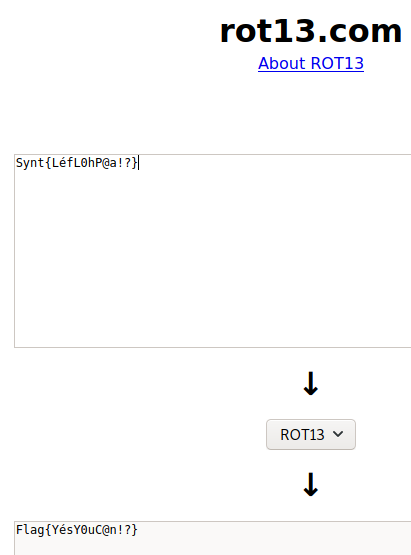
\includegraphics[width=0.5\linewidth ]{images/Robbe/sniffer_1.png}
\end{center}
\pagebreak
The other part of the hint is that a rotten algorithm (so using a ROT encryption method) doesn't change all characters. You can't search on "Flag" or something like that, but you can search for an accolade as this doesn't change. We simply convert this word document back to a pdf file and we have our first task completed.

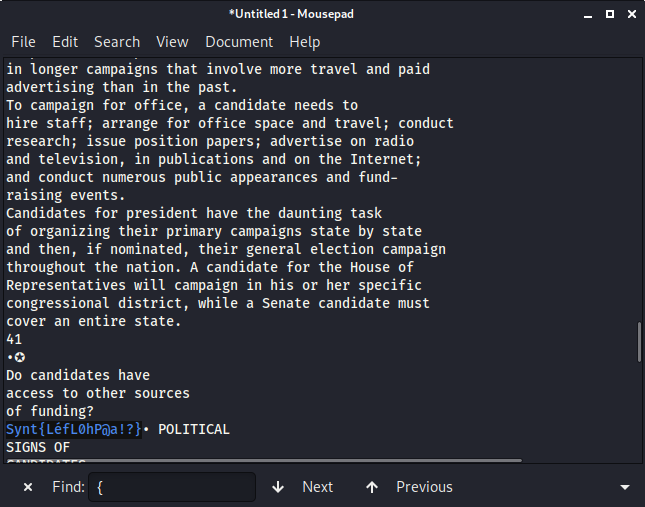
\includegraphics[width=\linewidth]{images/Robbe/sniffer_2.png}

\pagebreak
\textbf{\textit{Mysterious Image}}

Then the second part, the creation of our image. The idea is to create a hidden text file inside an image. In order to implement this idea, I used the tool Steghide. This is a steganography program that I used in previous CTF's. After searching online I found a decent picture that illustrates the Elections. Important is that it was a JPG-formatted image as Steghide only works with this kind of illustrations. The second step is to create a 'secret.txt' file in which we put a base64-encoded fake flag. 

\begin{center}
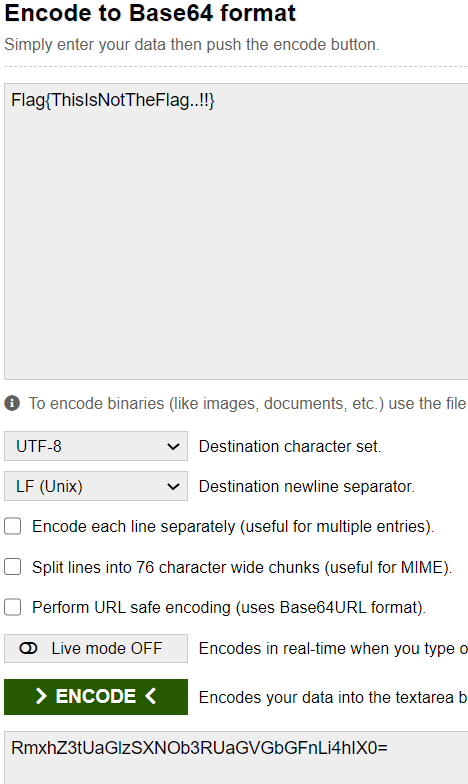
\includegraphics[width=0.5\linewidth]{images/Robbe/sniffer_3.png}
\end{center}
\begin{lstlisting}
echo "RmxhZ3tUaGlzSXNOb3RUaGVGbGFnLi4hlX0=" >> secret.txt
\end{lstlisting}

\pagebreak
After that, we use Steghide to embed the 'secret.txt' in the picture. The command will ask for a passphrase but we leave it empty in this challenge. To make sure the secret text file is added correctly, we can use the "info" parameter as you can see in the picture below.

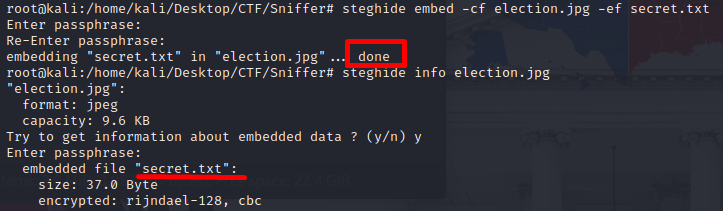
\includegraphics[width=\linewidth]{images/Robbe/sniffer_4.png}

\textbf{\textit{The intercepted Russian secret}}

So at this point, we have our two files created and we begin at the last part, creating the email. As we create this CTF for a school project, we used our student mail to simulate the IT department's conversation. In the picture below you can find the email. Of course, to use it in our CTF we need to download it as an eml file. In previous experiences with CTF's, I found that this was quite a challenging file format. With the package \textit{"mpack"} you can extract files from the downloaded email. 
\begin{center}
    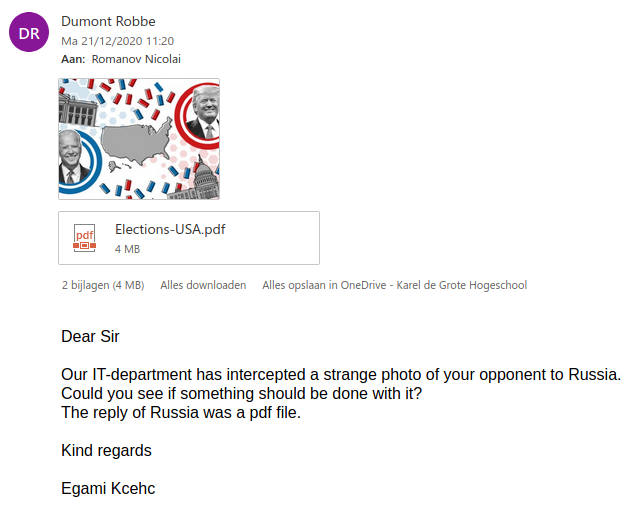
\includegraphics[width=0.7\linewidth]{images/Robbe/sniffer_5.png}
\end{center}

If you look closer, you can find an important hint in the email (look for the name).
That's basically how I created this challenge. I think this is a medium level challenge and is pretty doable for everyone with the right search on the internet.

\pagebreak

\subsubsection{Write up}
To start the challenge, you download the Sniffer.eml file from our online platform. It is important to always carefully examine the little story of the challenge, as well as the hint. In this case, I didn't notice anything special about the story, so I just downloaded the eml file.
 \begin{center}
    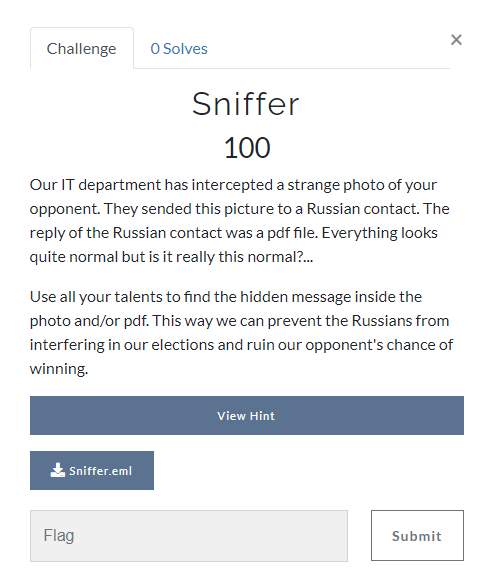
\includegraphics[width=0.5\linewidth]{images/Robbe/sniffer_writeup1.png}
\end{center}
Then I took a moment to think carefully about the hint. It's about the fact that some things don't change with a rotten algorithm. What I understand from this, is that - at some point - this challenge will use ROT encryption.
 \begin{center}
    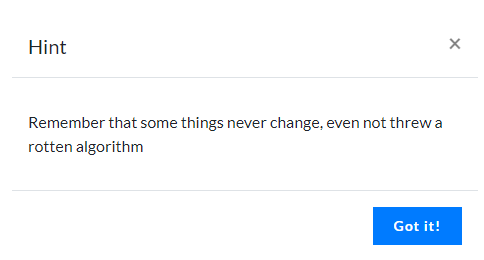
\includegraphics[width=0.5\linewidth]{images/Robbe/sniffer_writeup2.png}
\end{center}

\pagebreak
As I've got a bit of experience with the "mpack" package, I knew that with the \textbf{\textit{munpack}} command I can extract files from an email. Ofcourse to get to this point I tried multiple things but nothing else worked. With a quick look on Google, you'll find the "mpack" package and all its options. The following images will give you a look of how to use the package and in what this results:
\begin{figure}[h]
\begin{subfigure}{0.5\textwidth}
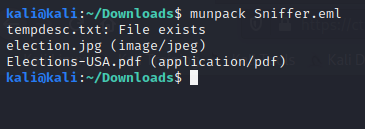
\includegraphics[width=1\linewidth]{images/Robbe/sniffer_writeup3.png}
\caption{Extract files from email with "mpack"}
\end{subfigure}
\begin{subfigure}{0.5\textwidth}
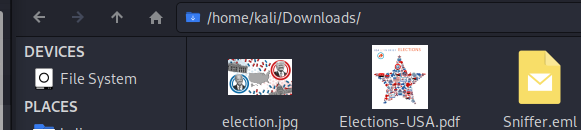
\includegraphics[width=1\linewidth]{images/Robbe/sniffer_writeup3b.png}
\caption{Results in these files}
\end{subfigure}
\end{figure}

 A good preparation for a CTF is always to look at and study the right tools for the right categories in advance. By doing this, you'll also come across the Steghide tool during your preparation. This is a steganography program with which you can very easily extract hidden data from a JPG illustration. So the fact that in this challenge we have to search for info from a JPG picture already rang a bell with me that we could probably use Steghide. The Steghide command will ask for a passphrase. As I had no idea what this could be, I pressed enter and apparently no password was set. The extracted data is written to a text file in which we then find an encrypted string. 

 \begin{center}
    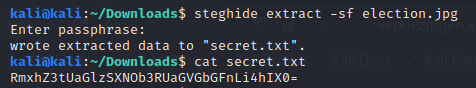
\includegraphics[width=1\linewidth]{images/Robbe/sniffer_writeup6.png}
\end{center}

\pagebreak
The first encryption method I tried was the Base64 format. Online there are many tools available to decrypt the string. Unfortunately, we have wasted a bit of our time examining the image as we found a fake flag. 
 \begin{center}
    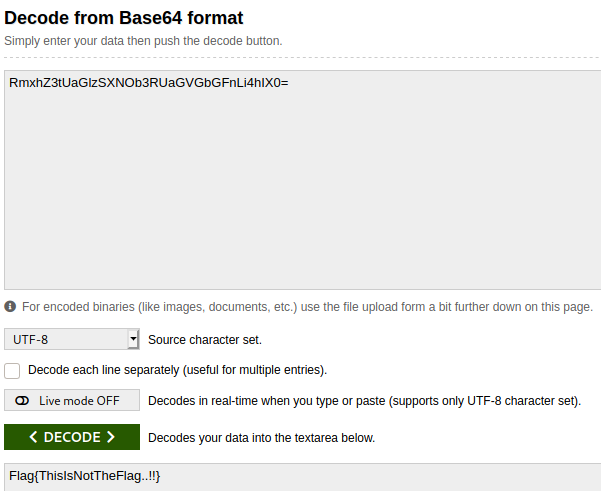
\includegraphics[width=0.5\linewidth]{images/Robbe/sniffer_writeup7.png}
\end{center}

With this little disappointment behind us, we jumped on the pdf. From previous experiences with Capture the Flag's, I knew that people often simply add data to a pdf but in blank font colour. To explore this easy option you simply open the pdf, press CTRL + A and copy all the data to a text editor. But then the real challenge starts, now look for a flag in all these data... 

At the time, I remembered the hint that a rotten algorithm does not change everything. With the help of my best friend Google, I found that a ROT encryption is going to change all the characters outside of an accolade. SO by searching on an accolade we find our encrypted string. 
 \begin{center}
    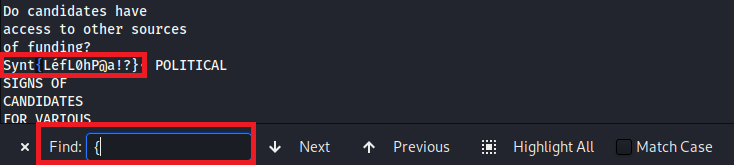
\includegraphics[width=1\linewidth]{images/Robbe/sniffer_writeup4.png}
\end{center}

Of course, we still need to find out which ROT encryption was used. The most obvious choice would be to go through all the ROT methods one by one, starting with ROT1, but this is very time-consuming. Instead, I started with the best-known ROT encryption, ROT13.
 \begin{center}
    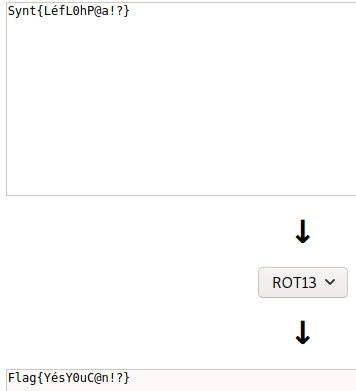
\includegraphics[width=0.5\linewidth]{images/Robbe/sniffer_writeup5.png}
\end{center}

So with a bit of luck we saved a lot of time and still found the right flag. The first Forensics challenge is already completed.
 \begin{center}
    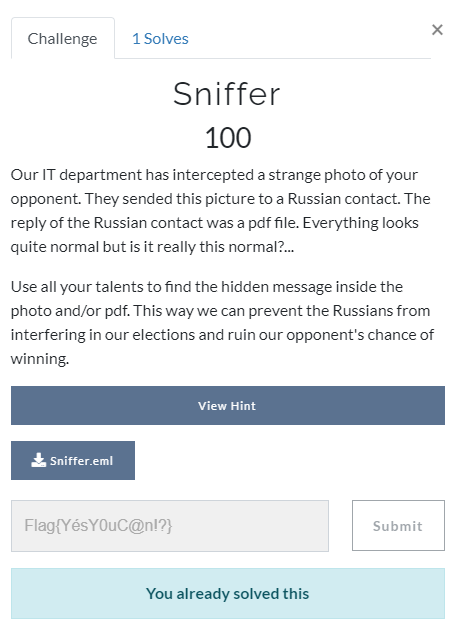
\includegraphics[width=0.5\linewidth]{images/Robbe/sniffer_writeup8.png}
\end{center}
\pagebreak

\subsection{Sniffer2}
With the "Sniffer2" challenge, the goal is to intercept the important flag of California. 

The person in charge of the voting office in the State of California was involved in many other things during his service than simply checking the votes. However, we also suspect that this person is manipulating the votes to our disadvantage...

In order to prove this, I intercepted his network traffic during his shift. While he went to the toilets I sneaked into his office and I saw an interesting zip file on his laptop's desktop. Just in time, I copied this file onto my laptop. Now it's up to you to find his big secret.

\subsubsection{Challenge explained}

For this challenge, you will receive an interesting zip file and the network traffic of the responsible person. The aim is to find what the person was doing during his shift. If you find what he was doing, you can find his username and password combination. With his credentials, you can start to put your attention on the zip file. Hopefully, you'll find his big secret.

\subsubsection{Creation Write up}
After a quick look, I found a pcap file of some network traffic. In this file, I found an HTTP POST request to log in with his credentials. To fill up the pcap file, I created a second pcpap with some other requests. Then I simply merged these two files together using the tool \textit{\textbf{mergecap}}.

\begin{lstlisting}
mergecap -w sniffer2.pcapng online_capture.pcapng http_post_request.pcapng
\end{lstlisting}

After that, I created my password-protected zip file. The password is the one you found minutes before with the login request. First, I made a directory, called "SeCrEtKeY", in which I putted a text file (SniffieSnif). Inside the text file is an encrypted string as you can see in the following screenshot. This string is the encryption of our flag (Flag{IC@nW!n}), using the Twofish algorithm. Important is to use a secret key to be able to encrypt and later decrypt this hash. The secret key is really easy as it is the name of the folder in our zip file. We perform this encryption using an online encryption tool which supports the Twofish algorithm.

\begin{lstlisting}
mkdir SeCrEtKeY
cd SeCrEtKeY
echo "aRFByuf8TLr6heCr2Nt3OpgHrsUVNKOFeNPOzNestcE=" >> SniffieSnif
\end{lstlisting}

 \begin{center}
    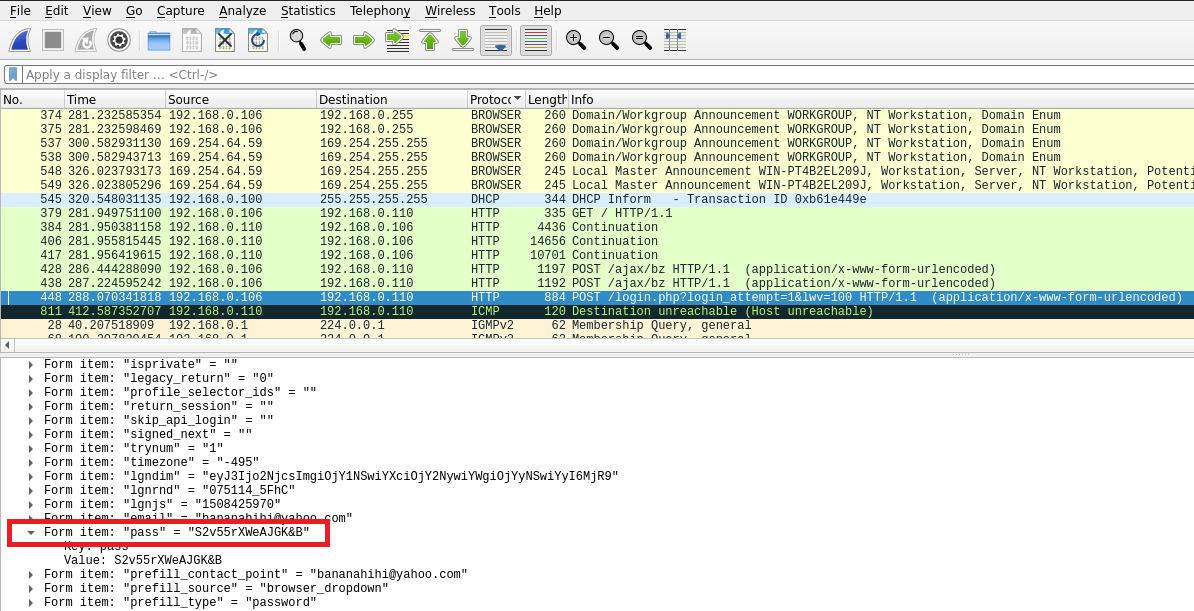
\includegraphics[width=1\linewidth]{images/Robbe/sniffer2_2.png}
\end{center}

\subsubsection{Write up}
On the online platform, you'll find the instructions of "Sniffer 2", where you can download a zip file. From the story we can conclude that we have to look for what this person just did on his laptop. This activity will bring us closer to the flag. Then we also have a zip file that we have to investigate. So my first thought is that, based on the pcap file, we will find the flag within the zip file.

 \begin{center}
    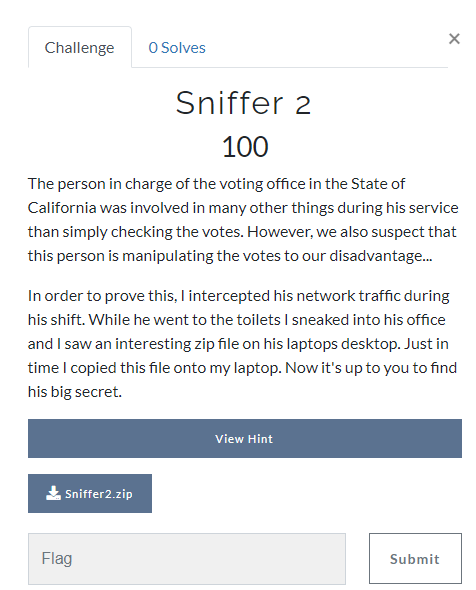
\includegraphics[width=0.5\linewidth]{images/Robbe/sniffer2_writeup1.png}
\end{center}

\pagebreak
At the moment, the hint does not really seem to add any value. Hopefully, further on in this challenge, it will become clear what exactly this will mean.
 \begin{center}
    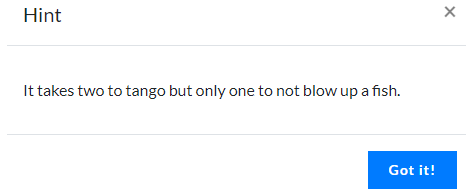
\includegraphics[width=0.5\linewidth]{images/Robbe/sniffer2_writeup2.png}
\end{center}

The first step is to unzip the downloaded zip file. When we do this the system will ask for a password for a "SniffieSnif" file. Since we don't have any clue of what the password this file can be, the file will not be handled and we'll only get a pcap file.
 \begin{center}
    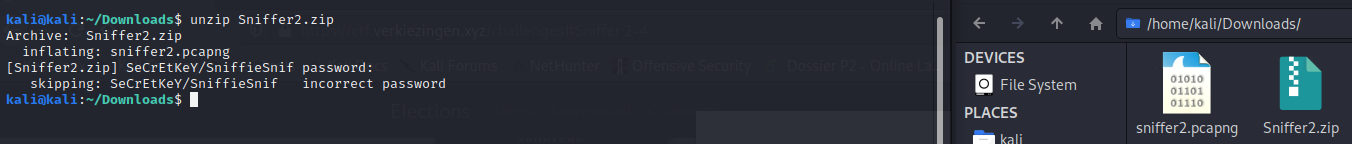
\includegraphics[width=1\linewidth]{images/Robbe/sniffer2_writeup3.png}
\end{center}

So, as I thought, we should be able to use our pcap to continue working on the archived directory containing the "SniffieSnif" file.
Studying a pcap takes a lot of time and using a lot of filters. One filter that revealed the secret of the employee was the "http" filter. This leaves us with seven requests, the first of which immediately got my attention. What we see here is a POST request to log in. If we look at this request in detail, we find the credentials that this official used.
Maybe with this password, we can also unpack his zip file. In the picture below you can see in the terminal that we run the \textbf{\textit{unzip}} command again and enter "S2v55rXWeAJGK&B" as the password. Our thoughts were completely correct and we get a new directory (SeCrEtKeY) containing the SniffieSnif file.

 \begin{center}
    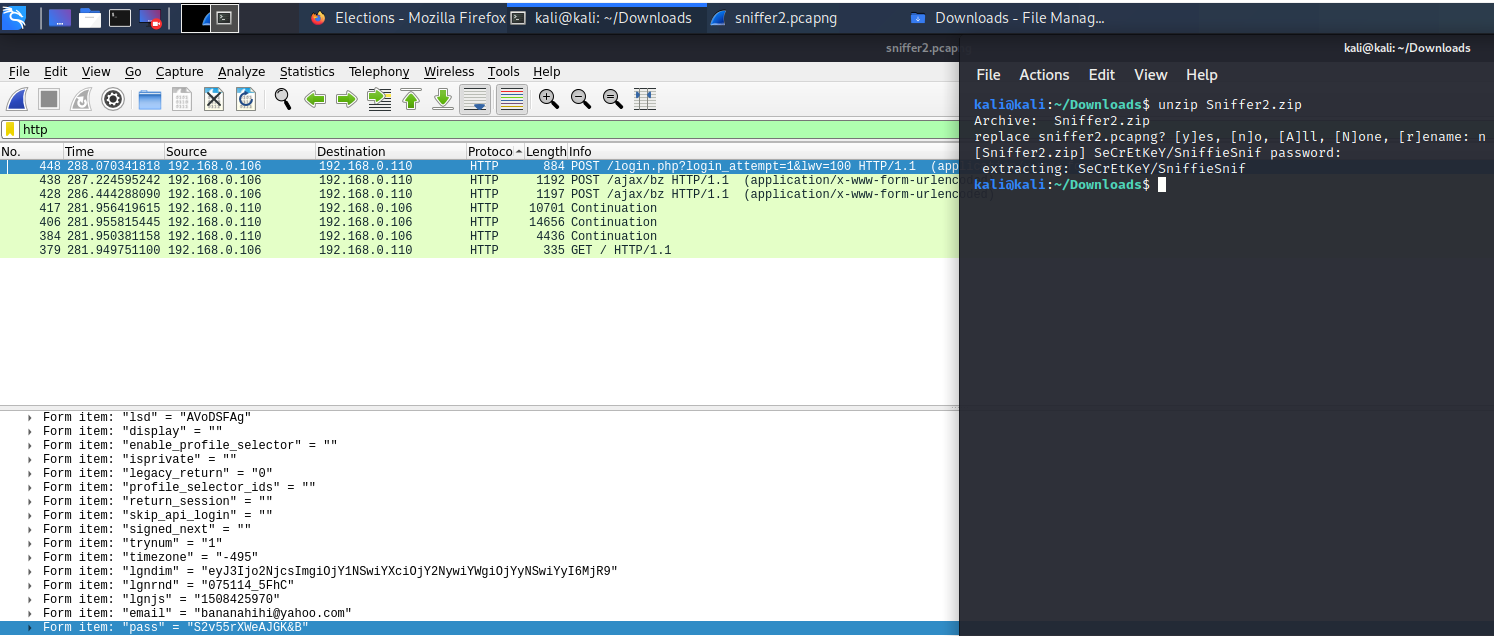
\includegraphics[width=1\linewidth]{images/Robbe/sniffer2_writeup4.png}
\end{center}

\pagebreak
In the "SniffieSnif" file we find an encrypted string. After a long search, using for example the tool "hashid", I still couldn't find which method was used here. 

Then I went back to the hint and thought about it a bit more carefully. What struck me were the words "blow" and "fish", as there is an encryption method called Blowfish. Using some online tools I tried to decrypt it this way but without much success. 

Importantly, the hint also contains the word "not". There is also an emphasis on the fact that you have to be with two to dance the tango. If we combine this, we come to the Twofish algorithm. Twofish does need a key to decrypt its hash... What had struck me before was the name of the archived folder (SeCrEtKeY). By playing a bit with the modes, we finally found our flag.
 \begin{center}
    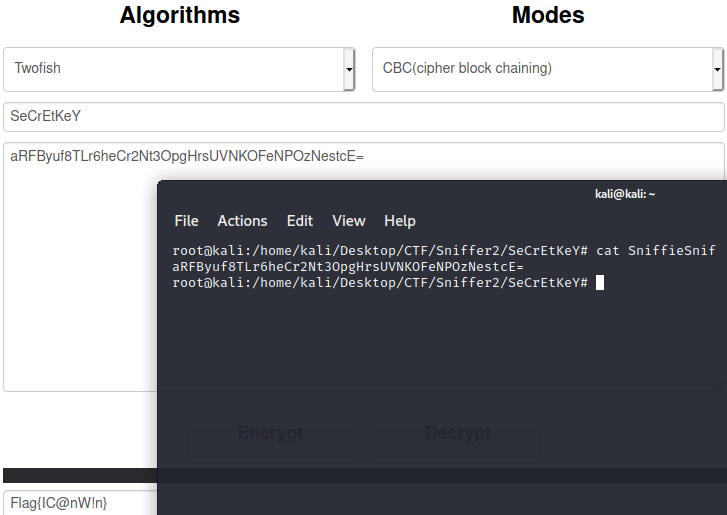
\includegraphics[width=1\linewidth]{images/Robbe/sniffer2_1.png}
\end{center}

\pagebreak
What I've found, however, is that there are relatively few online tools that can decrypt the Twofish algorithm correctly. A possible solution for this is to run a python script, such a script can be found online quite easily. This challenge was therefore fairly simple in terms of techniques, but it's still quite time-consuming due to the search in the pcap and the more difficult decrypting of a Twofish hash.
 \begin{center}
    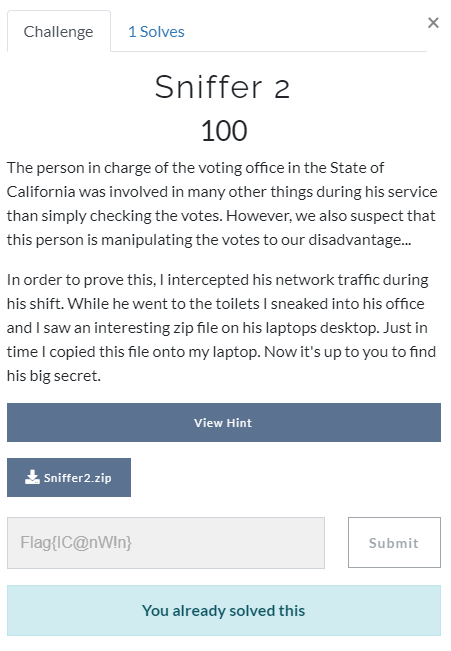
\includegraphics[width=0.5\linewidth]{images/Robbe/sniffer2_writeup5.png}
\end{center}
 

\pagebreak
\subsection{Sorry, wasn't meant for you}
With the "Sorry, wasn't meant for you" challenge, it's the goal to find the hidden flag inside of a couple of images.

Your presidential candidate's marketing guy worked out some images for our campaign. It looks like your favourite wants to send a secret message to his followers. 

Using all your skills and imagination will help you find that secret message. Maybe you're just in time to find his secret and help him win the election.

\subsubsection{Challenge explained}
For this challenge, I used two hiding techniques for inside images. The first one is based on a couple of easy Linux command line commands and the second one uses a well-known steganography tool to hide files inside images. Together with an easy encryption method, I finalised this task.
 
\subsubsection{Creation Write up}

\textbf{\textit{Method 1}}

As a start, I searched for a nice picture relating to the US Elections. After that, I created a directory "Sorry" where I saved this image. Inside this dir, I created another directory in which I putted a "Flag.txt" file. This flag file doesn't contain the real flag but does contain the password for a step later on. The aim is to embed the fake flag inside our image. It sounds difficult, but in the end, it's just creating an archive of our directory and then using the \textbf{cat} command to concatenate the archive with our image and save the output.

Our starting point is a directory with an image. The next steps will create an extra dir with a text file with inside a fake encrypted flag, an archive of this folder and in the end merge the zip file into our image:
\begin{lstlisting}
mkdir secret
cd secret
touch flag.txt
\end{lstlisting}

As an encryption method, we use the very well-known Base64 format in this challenge. Numerous tools can be found online that can encrypt and decrypt this format. After encrypting our fake flag, we putted our string into the flag.txt file. After adding our fake flag, we archived this directory (\textit{secret}) into \textbf{secret.zip}.
\begin{center}
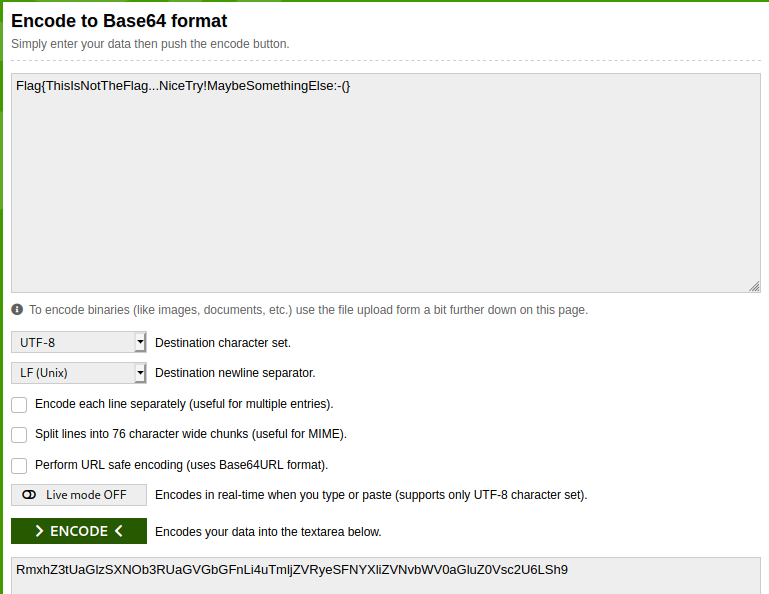
\includegraphics[width=1\linewidth]{images/Robbe/sorry1.png}
\end{center}
\begin{lstlisting}
cat image1.jpg secret.zip > secret.jpg
\end{lstlisting}
With the \textbf{cat} command above, we embedded our archived directory into the image. The secret.jpg file will look like an ordinary photo but contains our zip. That's how easy it is to complete our first method.

\pagebreak
\textbf{\textit{Method 2}}

For the second method, I used the open-source steganographic tool \textbf{\textit{Stegosuite}}. This is a tool that I used in earlier CTF's and is a really powerful and easy-to-use graphical tool. Just launch Stegosuite and you can insert an image via \textbf{File - Open}. So I searched for a second image (\textit{image.jpg}) and saved it into our "Sorry" folder. Finally, we also have to create a flag.txt file, where we store the real flag. Just like the other flag, we'll use the Base64 format.

\begin{lstlisting}
cd Desktop/CTF/Sorry
mkdir secret2
cd secret2
\end{lstlisting}
\begin{center}
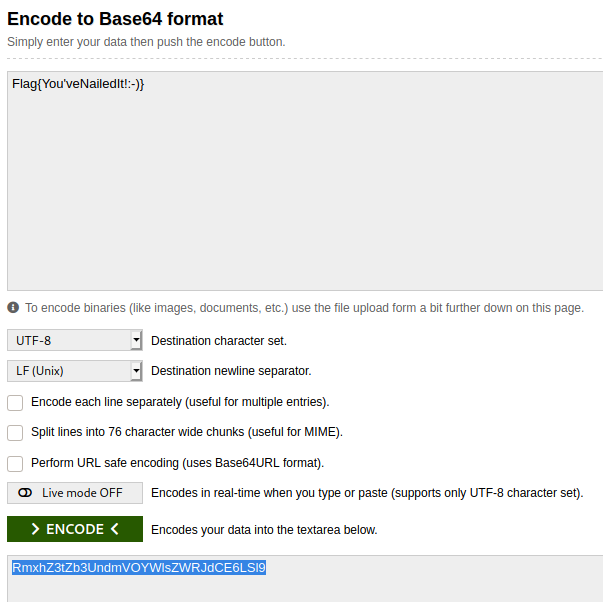
\includegraphics[width=1\linewidth]{images/Robbe/sorry3.png}
\end{center}
\begin{lstlisting}
echo "RmxhZ3tZb3UndmVOYWlsZWRJdCE6LSI9" > flag.txt
\end{lstlisting}

\pagebreak
Then we come to the Stegosuite-section: To open this graphical tool type in the command line "stegosuite" after which the program will open. Add the second photo via the "File" tab. In Stegosuite, the first option is there so that you can add an optional message. Secondly, we right-click in the second form to add our flag.txt. The last part is to give it a password. Our password is the fake flag from part one, so as a password we took \textit{"Flag\{ThisIsNotTheFlag...NiceTry!MaybeSomethingElse:-(\}"}. Then it is just a simple case of clicking on the "Embed" button and our secret is safely stored in the image.

That was again a very nice challenge to make using a few simple tools. We just have to put these two images in a zip file and this challenge has been completed.

\subsubsection{Write up}
As with the "Sniffer 2" challenge, we can download a zip on the online CTF platform containing all the necessary files. After reading the story, it is clear that this isn't really a pure Forensics challenge, but this is more the study of some images.

 \begin{center}
    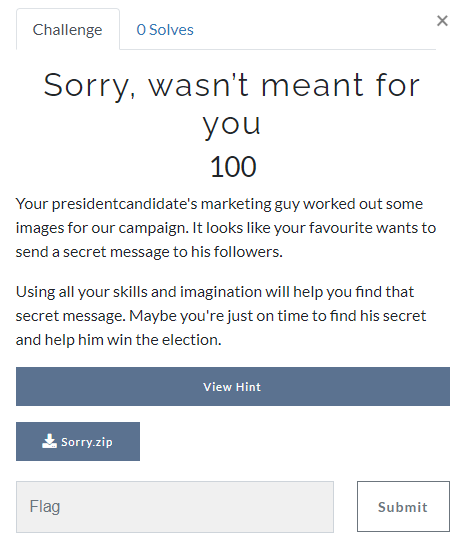
\includegraphics[width=0.6\linewidth]{images/Robbe/sorry_writeup1.png}
\end{center}

\pagebreak
The hint in itself is not really an added value as IT professionals always have to learn to use the right tools. CTF challenges are usually not particularly difficult if you have the knowledge of the right techniques, tools and protocols. The difficulty for beginning CTF'ers is therefore in learning these things.
\begin{center}
    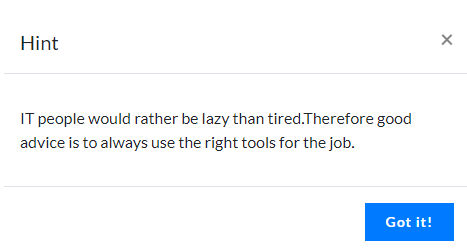
\includegraphics[width=0.6\linewidth]{images/Robbe/sorry_writeup2.png}
\end{center}

Our starting point is a zip file, so of course, we're going to unpack this packet first. In order to continue working with the hidden data in our first image, we first have to unzip it. Of course, you will not get to this step directly, but by using the command "file" and many others, you can see that there are hidden files in this picture. Since zipping files into a photo is a frequently used technique, we try to solve this problem using the archive function. 

After unzipping the image, we see that a folder is created with a flag.txt file in it. This text file contains an encrypted hash.
\begin{center}
    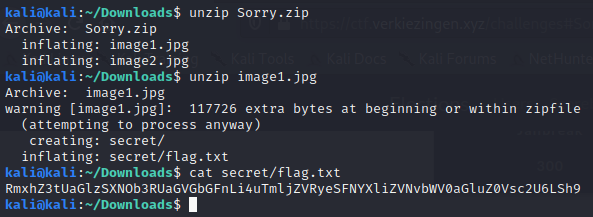
\includegraphics[width=1\linewidth]{images/Robbe/sorry_writeup3.png}
\end{center}

\pagebreak
The outcome of our decryption is, of course, disappointing as this is not the right flag ... What is important is that this fake flag does say that it might be something else. So it's a good idea to remember this flag because maybe we are going to need it later on.
\begin{center}
    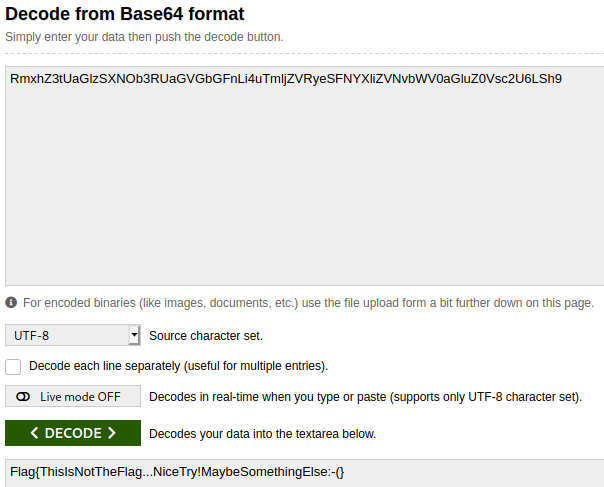
\includegraphics[width=0.8\linewidth]{images/Robbe/sorry_writeup4.png}
\end{center}

Then we arrive at the second photo: After the typical check whether the photo is actually a zip, I thought back to the hint. As an IT guy, you need to use the right tools, because that makes the work easier. A very well-known tool is Stegosuite, this makes it very easy to extract or embed data in photos. 


So we open Stegosuite by entering the same-named command in our command line. At the tab "File" we enter our photo. Now we have to enter a password to extract possible data in this image. In the back of our mind was still the fake flag of the previous image and indeed this is the correct password. We see that a flag file has been found. This will also appear in the directory you are in the cmd. This file also contains an encrypted string.
\begin{center}
    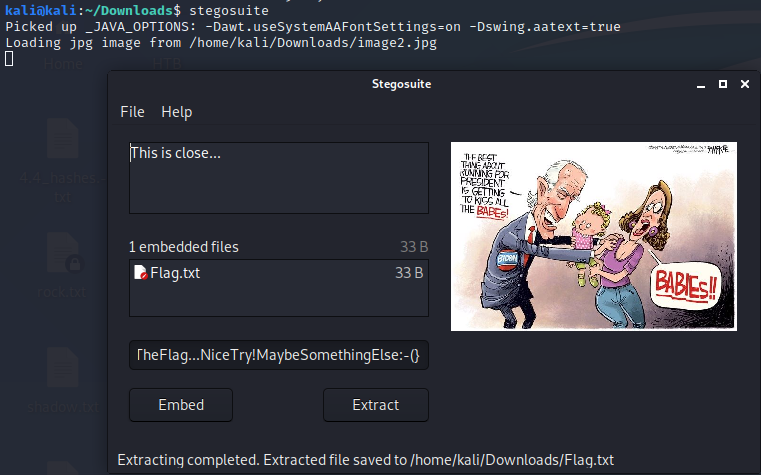
\includegraphics[width=1\linewidth]{images/Robbe/sorry_writeup5.png}
\end{center}

This string is also easy to decrypt with Base64. It looks like this is the flag we searched for.
\begin{center}
    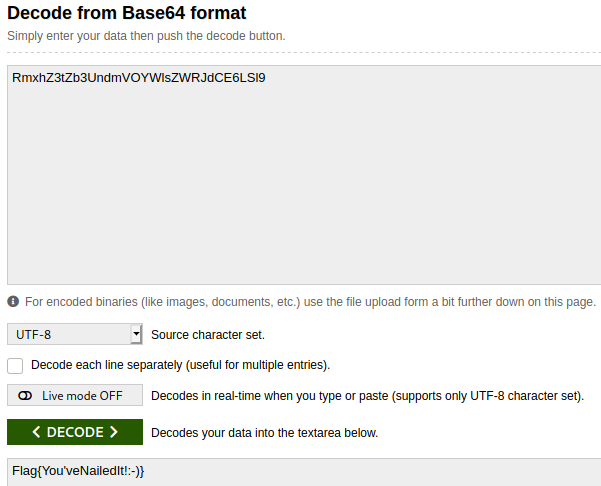
\includegraphics[width=1\linewidth]{images/Robbe/sorry_writeup6.png}
\end{center}

And indeed, the last flag we found is the correct one. So we have successfully completed all three challenges in the Forensics category.
\begin{center}
    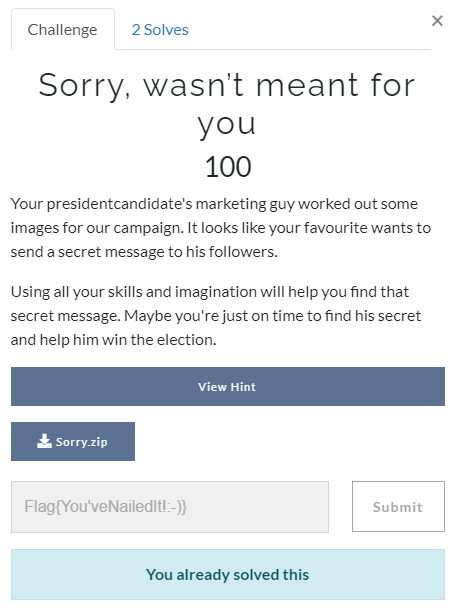
\includegraphics[width=0.6\linewidth]{images/Robbe/sorry_writeup7.png}
\end{center}
\end{document}